% prelude
% Copyright © 2018-2019 NextStep IT Training, a division of Smallrock Internet Services, Inc. All rights reserved.
%
% This document is the same course description and comments used for advertising the course, but is included
% in the book and slides so there is no misunderstanding of what will be addressed and the requirements.
%

\providecommand{\main}{..}
\documentclass[../workbook]{subfiles}
\graphicspath{ {\main/_Images/} }

\begin{document}

%% Course title and description, read from workbook-titles.tex

\section*{\bookcoursenumber \bookmajortitle}

Insert the course description here.


%% Class setup requirements.

\subsection*{Class Setup Requirements}

\begin{itemize}
    \item First requirement.
    \item Second requirement.
\end{itemize}


%% Participant prerequisites.

\subsection*{Prerequisites}

\begin{itemize}
    \item First prerequisite.
    \item Second prerequisite.
\end{itemize}


%% Course agenda (really just the chapter list).

\subsection*{Agenda}

\begin{itemize}
    \item Chapter 1 - Title
    \item Chapter 2 - Title
\end{itemize}


%% Facilities and etiquite (not labeled as such as to not offend anyone).

\subsection*{Facilities}

\begin{itemize}
    \item Please set your devices to vibrate in the classroom
    \item If you are on a conference bridge keep the connection muted unless you are talking
    \item The class has fixed hours and lunch, and there will be breaks; please be here on time
    \item Facilities: rest rooms, break rooms, coffee, vending, and refrigerators
\end{itemize}

\edef\measurepage{\the\dimexpr\pagegoal-\pagetotal-\baselineskip\relax}
\mbox{}\hfill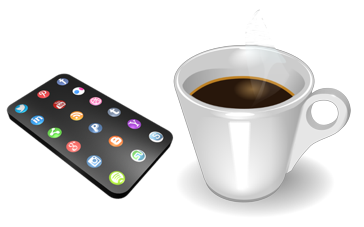
\includegraphics[keepaspectratio=true,height=\measurepage]{_Workbook/class-break}

\end{document}
